%!TEX program = xelatex
\documentclass[a4paper,UTF8]{article}
\usepackage{ctex}
\usepackage[margin=1.25in]{geometry}
\usepackage{color}
\usepackage{graphicx}
\usepackage{amssymb}
\usepackage{amsmath}
\usepackage{amsthm}
\usepackage{enumerate}
\usepackage{bm}
\usepackage{hyperref}
\usepackage{epsfig}
\usepackage{color}
\usepackage{mdframed}
\usepackage{lipsum}
\usepackage{graphicx}
\usepackage{float}
\usepackage{listings}
\lstset{language=Matlab}
\newmdtheoremenv{thm-box}{Theorem}
\newmdtheoremenv{prop-box}{Proposition}
\newmdtheoremenv{def-box}{定义}
\usepackage{listings}
\usepackage{xcolor}
\lstset{
	numbers=left,
	numberstyle= \tiny,
	keywordstyle= \color{ blue!70},
	commentstyle= \color{red!50!green!50!blue!50},
	frame=shadowbox, % 阴影效果
	rulesepcolor= \color{ red!20!green!20!blue!20} ,
	escapeinside=``, % 英文分号中可写入中文
	xleftmargin=2em,xrightmargin=2em, aboveskip=1em,
	framexleftmargin=2em
}
\lstset{numbers=left, 
numberstyle= \tiny, 
keywordstyle= \color{ blue!70},commentstyle=\color{red!50!green!50!blue!50}, 
frame=shadowbox, 
rulesepcolor= \color{ red!20!green!20!blue!20} 
} 


\usepackage{booktabs}

\setlength{\evensidemargin}{.25in}
\setlength{\textwidth}{6in}
\setlength{\topmargin}{-0.5in}
\setlength{\topmargin}{-0.5in}
% \setlength{\textheight}{9.5in}
%%%%%%%%%%%%%%%%%%此处用于设置页眉页脚%%%%%%%%%%%%%%%%%%
\usepackage{fancyhdr}
\usepackage{lastpage}
\usepackage{layout}
\footskip = 12pt
\pagestyle{fancy}                    % 设置页眉
\lhead{2021年春季}
\chead{模式识别}
% \rhead{第\thepage/\pageref{LastPage}页}
\rhead{作业四}
\cfoot{\thepage}
\renewcommand{\headrulewidth}{1pt}  			%页眉线宽,设为0可以去页眉线
\setlength{\skip\footins}{0.5cm}    			%脚注与正文的距离
\renewcommand{\footrulewidth}{0pt}  			%页脚线宽,设为0可以去页脚线

\makeatletter 									%设置双线页眉
\def\headrule{{\if@fancyplain\let\headrulewidth\plainheadrulewidth\fi%
\hrule\@height 1.0pt \@width\headwidth\vskip1pt	%上面线为1pt粗
\hrule\@height 0.5pt\@width\headwidth  			%下面0.5pt粗
\vskip-2\headrulewidth\vskip-1pt}      			%两条线的距离1pt
 \vspace{6mm}}     								%双线与下面正文之间的垂直间距
\makeatother

%%%%%%%%%%%%%%%%%%%%%%%%%%%%%%%%%%%%%%%%%%%%%%
\numberwithin{equation}{section}
%\usepackage[thmmarks, amsmath, thref]{ntheorem}
\newtheorem{theorem}{Theorem}
\newtheorem*{definition}{Definition}
\newtheorem*{solution}{Solution}
\newtheorem*{prove}{Proof}
\newcommand{\indep}{\rotatebox[origin=c]{90}{$\models$}}

\usepackage{multirow}

%--

%--
\begin{document}
\title{模式识别\\
作业四}
\author{181220076, 周韧哲, 本科,人工智能学院,人工智能学院选课}
\maketitle

\section*{Problem 1}
\begin{enumerate}[(a)]
	\item 
	    $\int_{-\infty}^{+\infty}p_1(x)dx=\int_{x_m}^{+\infty}\frac{c_1}{x^{\alpha+1}}dx=\frac{c_1}{\alpha}x_m^{-\alpha}=1$,故$c_1=\alpha x_m^\alpha$,容易看出$X$服从$\text{Pareto}(x_m,\alpha)$。
	\item 似然函数为$L(\alpha,x_m)=\prod_{i=1}^np(x_i|\alpha,x_m)$,易知样本满足$x_i\geq x_m$。则对数似然为$$LL(\alpha,x_m)=\sum_{i=1}^n\ln\frac{\alpha x_m}{x_i^{\alpha+1}}=n\ln\alpha+\alpha n\ln x_m-(\alpha+1)\sum_{i=1}^n\ln x_i$$
	求导
	\begin{align*}
	    \frac{\partial LL}{x_m}&=\frac{\alpha n}{x_m}\\
	    \frac{\partial LL}{\alpha}&=\frac{n}{\alpha} + n\ln x_m -\sum_{i=1}^n\ln x_i
	\end{align*}
	易知$\frac{\partial LL}{x_m}>0$,为了最大化对数似然,$x_m$要最大,因而$x_m=\min\{x_1,x_2,\cdots,x_n\}\doteq x_{min}$。令$\frac{n}{\alpha} + n\ln x_{min} -\sum_{i=1}^n\ln x_i=0$,得到$$\alpha=\frac{1}{\frac{1}{n}\sum_{i=1}^n\ln x_i - \ln x_{min}}$$
	所以最大似然估计为$x_m=x_{min},\alpha=\frac{1}{\frac{1}{n}\sum_{i=1}^n\ln x_i - \ln x_{min}}$。
	\item 由贝叶斯定理,当$\theta\geq x_m$时:
	\begin{align*}
	    p(\theta|D)&=zp(D|\theta)p(\theta|x_m,k)\\
	    &=z\prod_{i=1}^n\frac{1}{\theta}\times f\frac{kx_m^k}{\theta^{k+1}}\\
	    &=\frac{zkx_m^k}{\theta^{n+k+1}}
	\end{align*}
	其中$z$为规范化因子。由$\int_{-\infty}^{+\infty}\frac{zkx_m^k}{\theta^{n+k+1}}d\theta=1$得到$z=\frac{(n+k)x_m^n}{k}$。所以
	$$p(\theta|D)=\frac{(n+k)x_m^n}{k}\cdot\frac{kx_m^k}{\theta^{n+k+1}}=\frac{(\theta+k)x_m^{\theta+k}}{\theta^{n+k+1}}$$
	当$\theta<x_m$时,$p(\theta|x_m,k)=0$,因而$p(\theta|D)=0$。所以,$p(\theta|D)=\frac{(\theta+k)x_m^{\theta+k}}{\theta^{n+k+1}}[\![\theta\geq x_m]\!]\sim\text{Pareto}(x_m,n+k)$。
\end{enumerate}

\section*{Problem 2}
\begin{lstlisting}
rng(0,'twister');
x = lognrnd(2,0.5,1000,1);
y = lognpdf(sort(x), 2, 0.5);
subplot(221); plot(sort(x),y); title('Real PDF');
[f,xi,bw] = ksdensity(x);
subplot(222); plot(xi,f);
title(['KDE with bw',mat2str(roundn(bw,-4))]);
[f,xi,bw] = ksdensity(x,'Bandwidth', 0.2);
subplot(223); plot(xi,f);
title(['KDE with bw',mat2str(roundn(bw,-4))]);
[f,xi,bw] = ksdensity(x,'Bandwidth', 5);
subplot(224); plot(xi,f);
title(['KDE with bw',mat2str(roundn(bw,-4))]);

x = lognrnd(2,0.5,10000,1);
[f,xi,bw] = ksdensity(x); disp(bw);
x = lognrnd(2,0.5,100000,1);
[f,xi,bw] = ksdensity(x); disp(bw);
\end{lstlisting}
\begin{enumerate}[(a)]
	\item 见上面代码第$2$行生成样本。
	\item 如下图所示,自动选择的带宽约为$0.9369$。
	\begin{figure}[H]
		\centering
		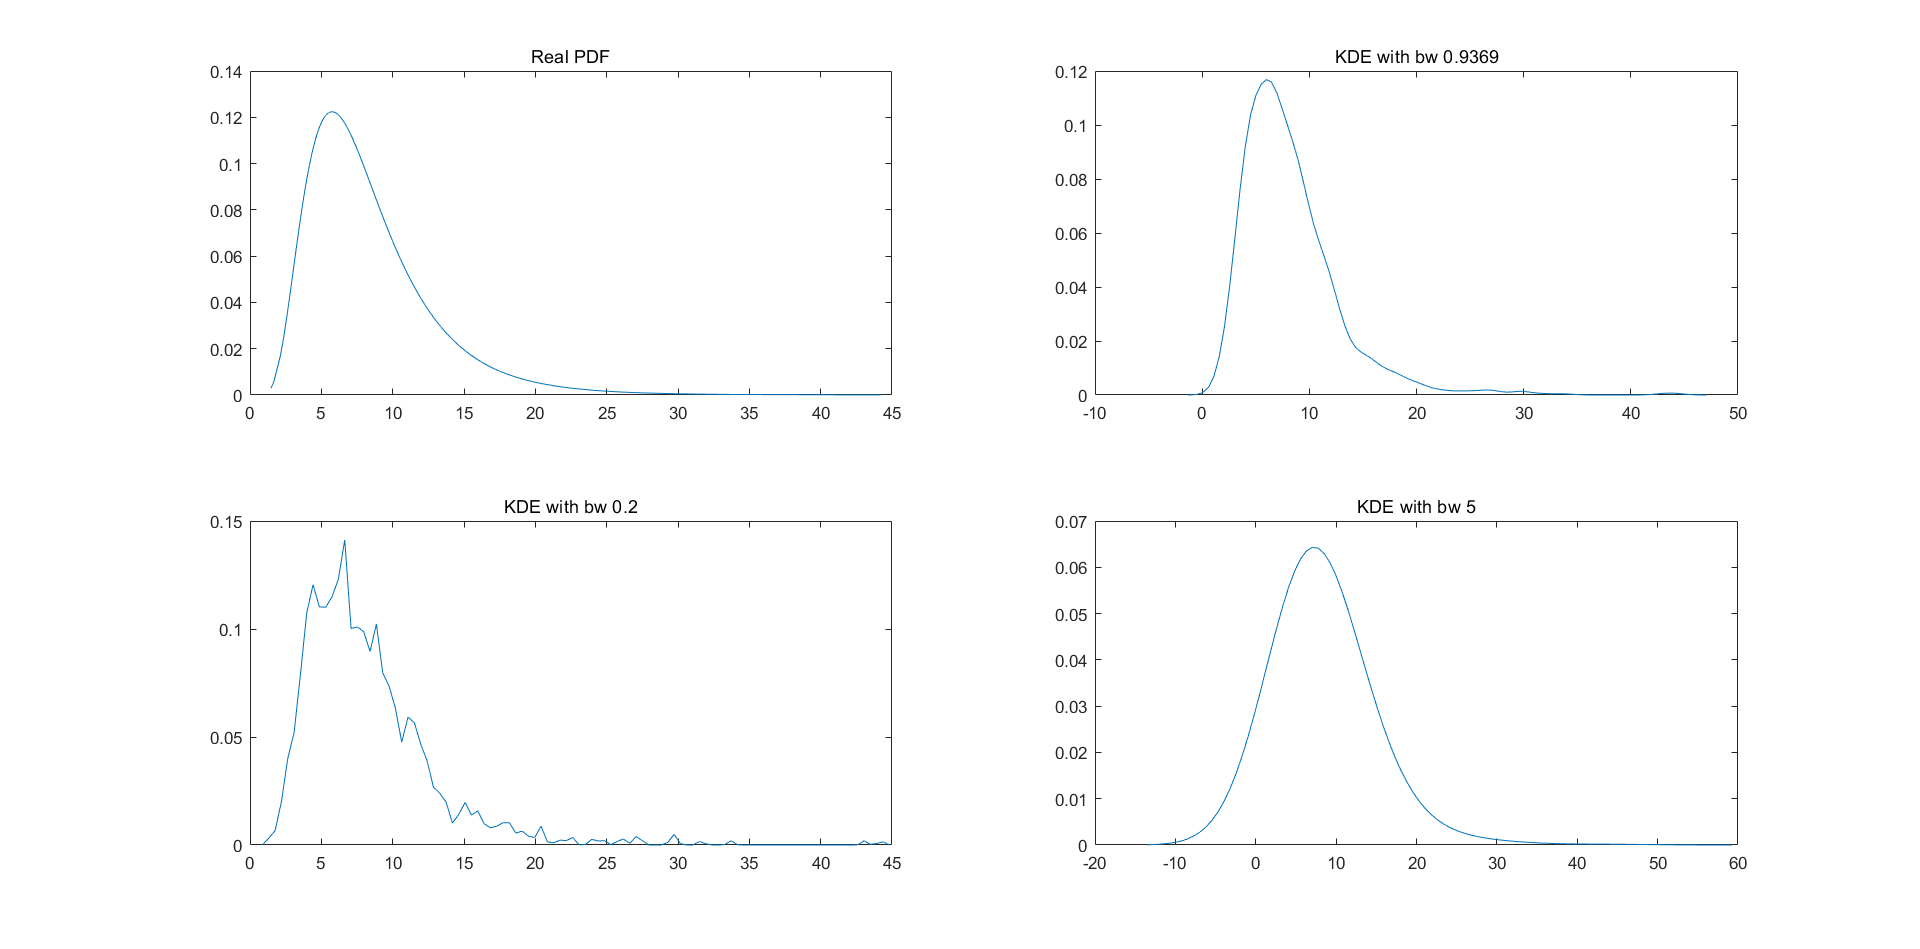
\includegraphics[width=1\textwidth]{pic/p2.png}
		\label{fig:2}
		\caption{P2}
	\end{figure}
	\item 如上图所示,带宽为$0.2$时生成的概率密度函数较陡峭,带宽为$5$时生成的概率密度函数更光滑。是带宽导致了这些曲线的差异,因为带宽反映了KDE曲线整体的平坦程度,随着带宽增大,KDE整体曲线就越平坦。
	\item 见上面代码第$15-18$行,$10000,100000$个样本对应的带宽分别为$0.5911,0.3805$,随着样本数增大,带宽逐渐减小。因为数据点越多,越容易拟合真实密度函数,这时小的带宽能让数据点在最终形成的曲线形状中所占比重更大,能更好地拟合真实密度函数。
\end{enumerate}

\section*{Problem 3}
\begin{enumerate}[(a)]
	\item 代码第一行使用带宽$H$,并且iSigma=$H^{-1}$。第二行定义了训练集,训练集实际上是两维的,即通过pts构造的temp,从而一共有$101^2$个二维样本。GT是个离散概率密度矩阵,即关于$101^2$个样本的离散概率密度,保存了手动计算的概率密度,并且在最后归一化了。
	\item 代码如下:
\begin{lstlisting}
pts = -5:0.1:5;
p1 = normpdf(pts, 0, 1.5);
p2 = normpdf(pts, 0, 2);
approximate = p1.'* p2;     %pdf的乘积来近似
approximate = approximate/(sum(approximate(:)));  %离散化
\end{lstlisting}
    \item 代码如下(接着(a)中的代码):
\begin{lstlisting}
best1 = 0; best2 = 0; min_error = 1;
for std1 = 0.05:0.05:3
    for std2 = 0.05:0.05:3
        p1 = normpdf(pts, 0, std1);
        p2 = normpdf(pts, 0, std2);
        MF = p1.'*p2; MF = MF/sum(MF(:));
        err = 1 - sum(min(GT(:),MF(:)));
        if err < min_error
            min_error = err;
            best1 = std1;
            best2 = std2;
        end
    end
end
disp("best std1: "+best1 + ", best std2: " ...,
+best2 +", distance: " + min_error);
\end{lstlisting}
运行代码得到两个标准差的最佳值分别为$1.35,1.95$,此时的最小距离为$0.11391$,即两个分布的距离较小,说明平均场近似是有用的。
\end{enumerate}

\section*{Problem 4}
\begin{enumerate}[(a)]
	\item $1,1,2, 3, 5, 8$。
	\item 将递归式写为:$F_n-F_{n-1}-F_{n-2}=0$,为二阶常系数齐次线性递推式,其特征方程为$\lambda^2-\lambda-1=0$,解为$\lambda_1=\frac{1+\sqrt{5}}{2},\lambda_2=\frac{1-\sqrt{5}}{2}$,从而$F_n=c_1\lambda_1^n+c_2\lambda_2^n$,由$F_1=F_2=1$得到:
	$$\left\{\begin{aligned}
c_1(\frac{1+\sqrt{5}}{2})+c_2(\frac{1-\sqrt{5}}{2}) = & 1 \\
c_2(\frac{1+\sqrt{5}}{2})^2+c_2(\frac{1-\sqrt{5}}{2})^2 = & 1 \\
\end{aligned}\right.$$
解得$c_1=\frac{1}{\sqrt{5}}, c_2=-\frac{1}{\sqrt{5}}$,所以
$$F_n=\frac{(\frac{1+\sqrt{5}}{2})^n-(\frac{1-\sqrt{5}}{2})^n}{\sqrt{5}}=\frac{\alpha^n-\beta^n}{\alpha-\beta}$$
    \item 证明:
    \begin{align*}
    \sum_{i=3}^{n+2}F_i&=\sum_{i=3}^{n+2}(F_{i-1}+F_{i-2})\\
                       &=\sum_{i=1}^{n}(F_{i}+F_{i+1})\\
                       &=\sum_{i=1}^{n}F_{i}+\sum_{i=1}^{n}F_{i+1}\\
                       &=\sum_{i=1}^{n}F_{i}+\sum_{i=3}^{n+1}F_{i} + F_2
    \end{align*}
    因此$\sum_{i=1}^{n}F_{i} =\sum_{i=3}^{n+2}F_i-\sum_{i=3}^{n+1}F_{i}-F_2=F_{n+2}-1 $。
    \item 首先有:$\sum_{i=j}^nF_i=F_{n+2}-1-\sum_{i=1}^{j-1}F_i=F_{n+2}-F_{j+1}$,则
    \begin{align*}
        \sum_{i=1}^niF_i &=\sum_{j=1}^n\sum_{i=j}^n F_i\\
              &=\sum_{j=1}^n(F_{n+2}-F_{j+1})\\
              &=nF_{n+2}-\sum_{j=2}^{n+1}F_{j}\\
              &=nF_{n+2}-(F_{n+3}-1-F_1)\\
              &=nF_{n+2}-F_{n+3}+2
              \end{align*}
    \item 容易得到离散概率分布为$p=\{\frac{1}{12},\frac{1}{12},\frac{1}{6},\frac{1}{4},\frac{5}{12}\}$。其霍夫曼树如下图所示。
        \begin{figure}[H]
		\centering
		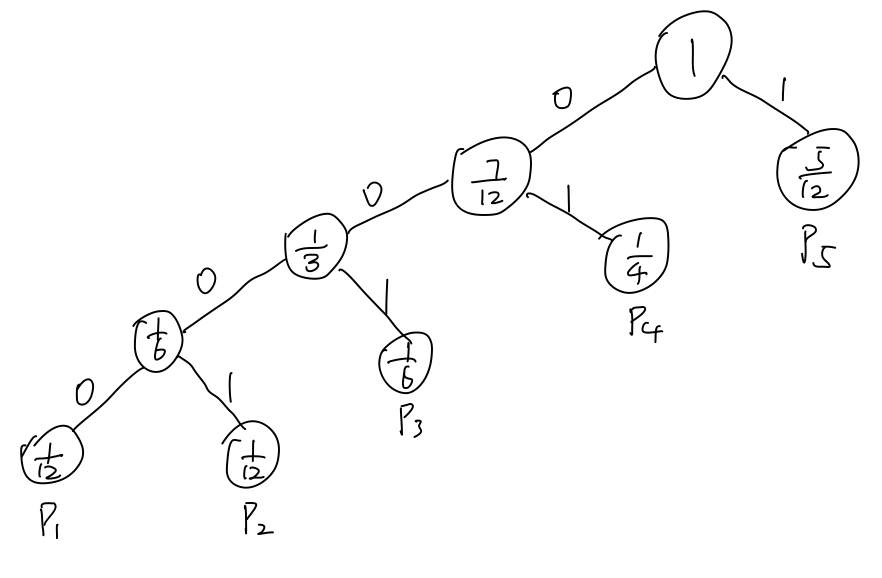
\includegraphics[width=0.5\textwidth]{pic/p4.png}
		\label{fig:1}
		\caption{霍夫曼树}
	\end{figure}
	更一般的情况下,$\frac{F_i}{F_{n+2}-1}(1\leq i\leq n)$的霍夫曼树是一棵结点数为$2n-1$,高度为$n$的二叉树,除了底层为两个叶结点之外,每一层都有且只有一个叶结点,且高度越高的叶结点对应的概率越大。这是因为第$i$个的概率总是比前$i-2$个的概率之和大,且比第$i-1$个的概率大:$F_i=F_{i-1}+F_{i-2}>F_{i-1},\quad F_i=F_{i+1}-F_{i-1}=\sum_{j=1}^{i-1}F_j +1- F_{i-1}=\sum_{j=1}^{i-2}F_{j +1}>\sum_{j=1}^{i-2}F_j$。
	\item 由(e)可知,$n>1$时,平均所需比特数为$\frac{F_1}{F_{n+2}-1}(n-1)+\sum_{i=2}^n\frac{F_i}{F_{n+2}-1}(n-i+1)$,此式可化简为:
	\begin{align*}
	    B_n&=\frac{(n-1)+\sum_{i=2}^nF_i(n-i+1)}{F_{n+2}-1}\\
	    &=\frac{-1+\sum_{i=1}^nF_i(n-i+1)-1}{F_{n+2}}\\
	    &=\frac{-1+\sum_{j=1}^n\sum_{i=1}^jF_i}{F_{n+2}-1}\\
	    &=\frac{-1+\sum_{j=1}^n(F_{j+2}-1)}{F_{n+2}-1}\\
	    &=\frac{-1+\sum_{j=3}^{n+2}F_{j}-n}{F_{n+2}-1}\\
	    &=\frac{-1+F_{n+4}-1-F_1-F_2-n}{F_{n+2}-1}\\
	    &=\frac{F_{n+4}-(n+4)}{F_{n+2}-1}
	\end{align*}
	\item $B_n=\frac{F_{n+3}-(n+3)+F_{n+2}-1}{F_{n+2}-1}=\frac{F_{n+3}}{F_{n+2}-1}-\frac{(n+3)}{F_{n+2}-1}+1$,因为$\frac{F_{n+1}}{F_n}=1+\frac{F_{n-1}}{F_n}$,令$f=\lim_{n\to\infty}\frac{F_{n+1}}{F_n}$,则得到$f=1+\frac{1}{f}$,解得$f=\alpha$(另一解小于0舍去)。所以:
	\begin{align*}
	    \lim_{n\to\infty}B_n&= \lim_{n\to\infty}\frac{F_{n+3}}{F_{n+2}-1}-\frac{(n+3)}{F_{n+2}-1}+1\\
	    &=1+\lim_{n\to\infty}\frac{1}{\frac{F_{n+2}}{F_{n+3}}-\frac{1}{F_{n+3}}}-\frac{(n+3)}{F_{n+2}-1}\\
	    &=1+\frac{1}{\frac{1}{\alpha}}-0\\
	    &=1+\alpha
	\end{align*}
	所以平均需要用$1+\alpha=\frac{3+\sqrt{5}}{2}$个比特来编码。
\end{enumerate}

\section*{Problem 5}
令$p(x)=\lambda e^{-\lambda x}(x\geq0,\lambda=\frac{1}{\mu})$,则$X$在$p(x)$下的熵为:
$$h(p)=-\int_0^\infty p(x)\ln p(x) dx=-\int_0^\infty \lambda e^{-\lambda x}\ln \lambda e^{-\lambda x} dx=\int_0^\infty\ln \lambda e^{-\lambda x} de^{-\lambda x}=1-\ln \lambda$$

我们先计算:
\begin{align*}
    -\int_0^\infty q(x)\ln p(x) dx
    &=-\int_0^\infty q(x)\ln \lambda e^{-\lambda x} dx\\
    &=-\int_0^\infty q(x)(\ln \lambda-\lambda x) dx\\
    &=-\ln \lambda\int_0^\infty q(x)dx +  \lambda \int_0^\infty xq(x) dx\\
    &=-\ln \lambda +\lambda \mathbb{E}[X]\\
    &=-\ln \lambda +\lambda\mu\\
    &=1 -\ln \lambda\\
    &= -\int_0^\infty p(x)\ln p(x) dx
\end{align*}

再计算$h(q)-h(p)$:
\begin{align*}
    h(q)-h(p)
    &=-\int_0^\infty q(x)\ln q(x) dx+\int_0^\infty p(x)\ln p(x) dx\\
    &=-\int_0^\infty q(x)\ln q(x) dx+\int_0^\infty q(x)\ln p(x) dx\\
    &=\int_0^\infty q(x)\ln \frac{p(x)}{q(x)} dx\\
    &\leq \int_0^\infty q(x)(\frac{p(x)}{q(x)}-1) dx\\
    &=\int_0^\infty p(x)dx - \int_0^\infty q(x) dx\\
    &=0
\end{align*}

从而,$h(q)\leq h(p)$,等号在$\frac{p(x)}{q(x)}=1$时成立,即参数为$\lambda=\frac{1}{\mu}$的指数分布是在这样约束条件下的最大熵分布。

\section*{Problem 6}
\begin{enumerate}[(a)]
	\item 证明:\begin{align*}
	   P(A,B|C)&=\frac{P(A,B,C)}{P(C)}\\
	           &=\frac{P(A)P(C|A)P(B|C)}{P(C)}\\
	           &=\frac{P(A,C)}{P(C)}P(B|C)\\
	           &=P(A|C)P(B|C)
	      \end{align*}
	 \item 证明:\begin{align*}
	   P(A,B|C)&=\frac{P(A,B,C)}{P(C)}\\
	           &=\frac{P(B)P(C|B)P(A|C)}{P(C)}\\
	           &=\frac{P(B,C)}{P(C)}P(A|C)\\
	           &=P(B|C)P(A|C)
	      \end{align*}
     \item 证明:\begin{align*}
	   P(A,B|C)&=\frac{P(A,B,C)}{P(C)}\\
	           &=\frac{P(A|C)P(B|C)P(C)}{P(C)}\\
	           &=P(A|C)P(B|C)
	      \end{align*}
	  \item 当$C$没有被观察到时:\begin{align*}
	   P(A,B)&=\sum_C{P(A,B,C)}\\
	         &=\sum_C P(A)P(B)P(C|A,B)\\
	         &=P(A)P(B)\sum_C P(C|A,B)\\
	         &=P(A)P(B)
	      \end{align*}
	      当$C$被观察到时,$A,B$不条件独立。一个直观例子是,令$A$表示学生努力程度,$B$表示课程难度,$C$表示考试成绩。在没有观察到考试成绩时,学生是否努力与课程难度显然是独立的。但当观察到考试成绩很高($A,B$的共同结果)的时候,$A$和$B$就会产生一些联系,例如如果努力程度低,那么课程难度很可能不难。
	  \item 观察到$C$的任意一个后代$F$后,这个观测会逆着从$C$指向$F$的箭头提供一些关于$C$的信息,因此会导致$A,B$仍然产生依赖。比如接着(d)的例子,令$F$代表妈妈是否给学生奖励。如果观察到妈妈给了奖励,那么可以知道考试成绩高,故$A$和$B$也产生了一些联系。
\end{enumerate}
\end{document}